\documentclass{IEEEtran}
\usepackage{graphicx}
\usepackage{hyperref}

\begin{document}

\title{ROBT 310 Image Processing - Project 3 Report}

\author{Anuar Maratkhan}

\maketitle

\section{Introduction}
This is the report for ROBT 310 project 2. The project is aimed to evaluate students' understanding of intensity transformations, spatial domain and frequency domain filtering. Students were given a noisy video customized personally for each student. Below I will describe the way I tackled the problem of denoising the video sequence.

\section{What has been done}
The video included four types of noises:
\begin{enumerate}
	\item salt-and-pepper noise
	\item periodic diagonal lines
	\item horizontal line moving from top to bottom of the video
	\item flicker noise
\end{enumerate}

According to that, I have divided my project intro three parts (denoising (3) and (4) are taken as one step).

\subsection{Salt-and-Pepper noise}
This part was easy enough and was implemented in one line programatically. I have used \textbf{median filter} for removing salt-and-pepper noise. And as it is shown in figure below, the filter has done its job very good.

\begin{figure}[h]
	\centering
	
\includegraphics[width=0.5\textwidth]{1.png}
\end{figure}

I have started to tackle the problem from the easiest one and firstly checked on one image. Later, rest of the filters were also applied like this: try on one frame of the video, apply to all video frames. Moreover, for application of filters on all frames I have used for loop iterating through all frames individually and applying the filter. The results of those filters I have written to another resultant video at the same iteration.

\subsection{Periodic diagonal lines}
The part with removing diagonal lines was the hardest from all because we had to apply our knowledge of signals in frequency domains and understand how to remove noises from frequency domain.

For this part, I have started with transforming one single video frame to frequency domain using MATLAB's \texttt{fft2} function (which corresponds to Fast Fourier Transform in 2-dimensions). To represent the frequency domain in more a convenient way I have shifted transformed image, took \texttt{abs} and \texttt{log} of that shifted image. From there I could see some bright spikes along a diagonal:

\begin{figure}[h]
	\centering
	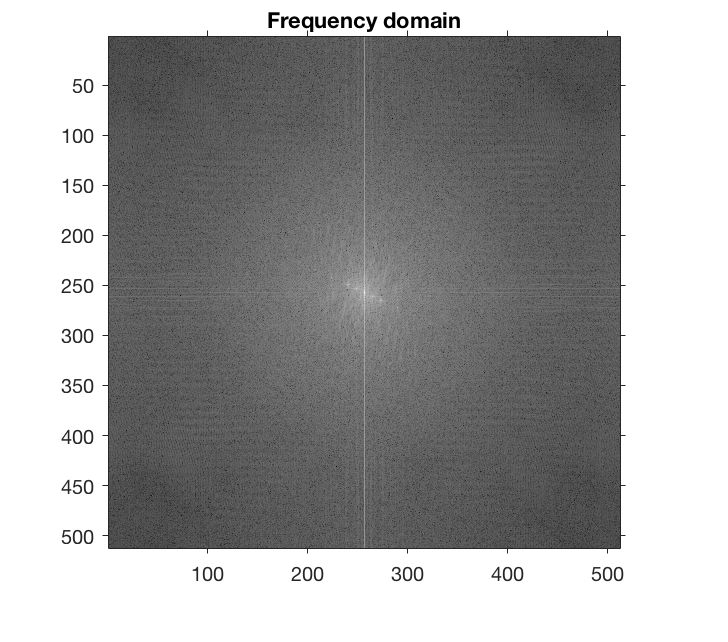
\includegraphics[width=0.3\textwidth]{frequency_domain.png}
\end{figure}

Further, I started taking only the highest values in the frequency domain by tresholding (intensity transformation). That step was very useful to find positions of brightest spikes in the frequency domain with MATLAB's built-in \texttt{axis on}.

With thresholding all frames in the video, I have obtained spikes that exist in each image. For that I have started with matrix all of ones of size [512, 512], which is the size of each frame, and multiplied it to each threshold result. Further, I have used it as a mask. The mask is included to the project directory.

Later, I have created a filter from that excluding the DC component lying at the center with neighbors in radius of 1 pixel. The filter then was multiplied to the original frequency domain. The resultant frequency domain is shown below (white in the image corresponds to zeroed values).

\begin{figure}[h]
	\centering
	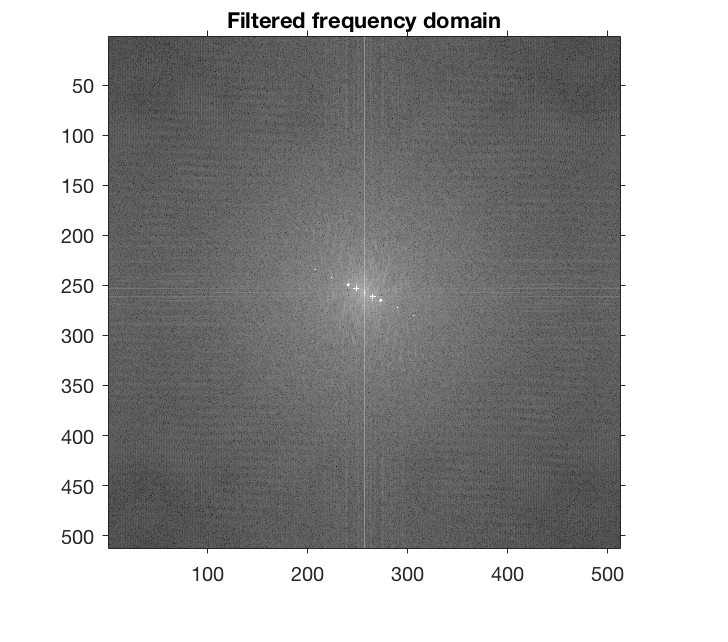
\includegraphics[width=0.3\textwidth]{filtered_frequency.png}
\end{figure}

After applying that filter to the frequency domain, I have taken inverse Fourier transform (with inverse shifting) using \texttt{ifft2} function. The result of inverse Fourier transform is shown below. The same was applied to all frames in the video. For convenience, I have written a separate function for that.

\begin{figure}[h]
	\centering
	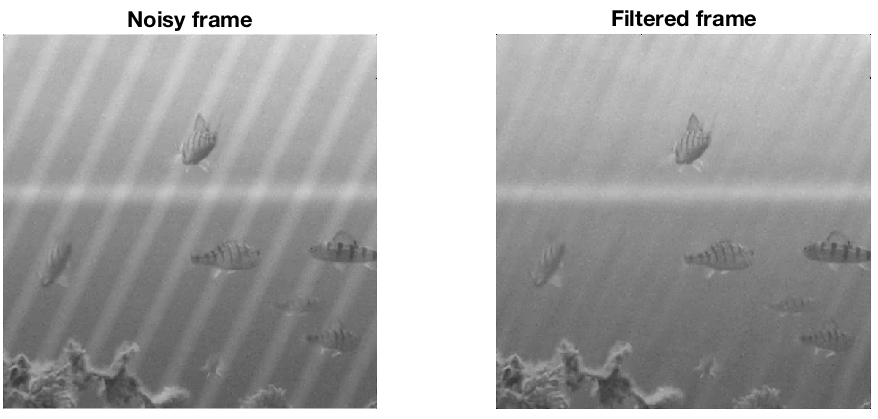
\includegraphics[width=0.5\textwidth]{2.png}
\end{figure}

\subsection{Moving horizontal line and flicker noise}
This part was the most interesting and brainstorming. I have added all video frames to one 3-dimensional matrix of size [512,512, \texttt{frames}]. Later I have replaced dimensions of the matrix by changing third dimension to the second, and the second to the third. The reason I have done it is because the horizontal line was moving along the second dimension as time passed. So roughly speaking I have changed time domain with OY domain of the video. From there, I started transforming each piece of the matrix (OX and time domain) to the frequency domain and observed another types of bright spikes.

\begin{figure}[h]
	\centering
	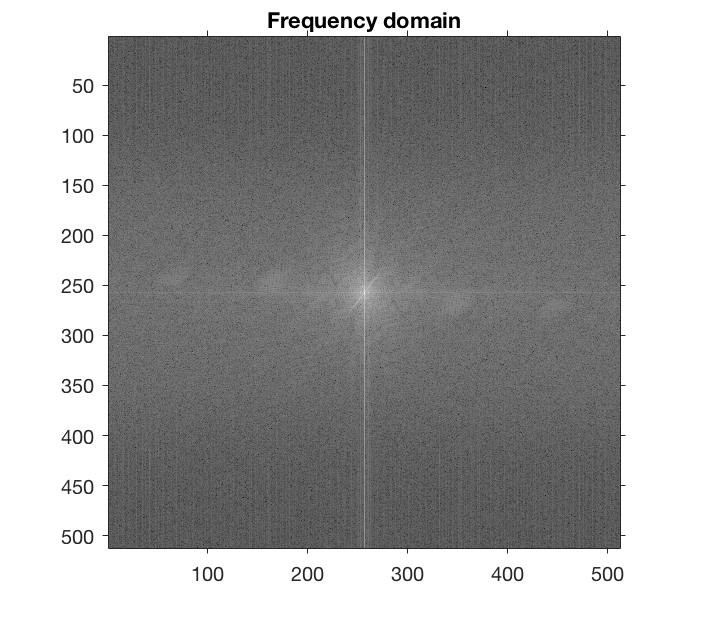
\includegraphics[width=0.3\textwidth]{time_domain.png}
\end{figure}

That frequency domain consisted of two types of noises: the horizontal line moving along OY which is a diagonal line of spikes in frequency domain, and flicker noise which is represented by two dots near the central DC component. The latter was easily removed by producing another filter (matrix of ones of the same size as frequency domain image), and zeroing those positions.

For the diagonal part in frequency domain I have decided to find two points along that diagonal line and find the equation of this line manually by algebraic calculations. As a result I have got an equation:

\begin{equation}
	y = -13/17*x + 7710/17
\end{equation}

But due to the short length of that diagonal line, I have applied it in the range of [237:277]. As a result, I have got filtered frequency domain of time domain.

\begin{figure}[h]
	\centering
	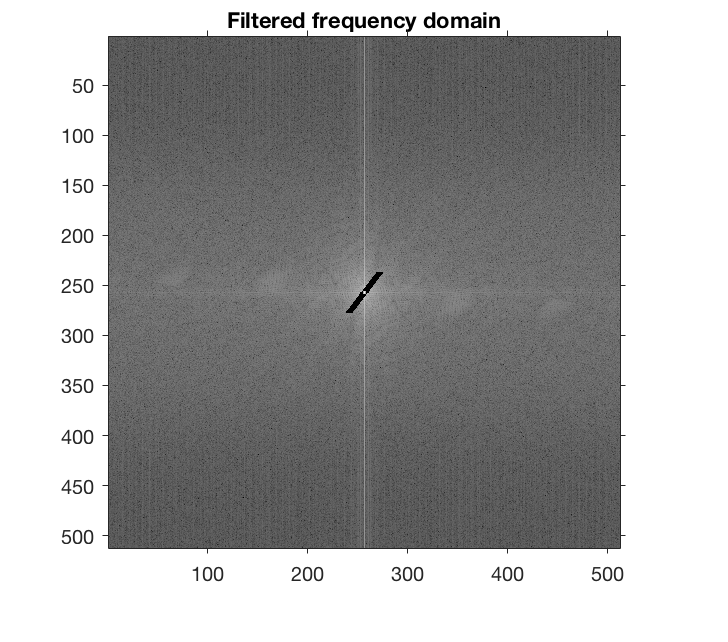
\includegraphics[width=0.3\textwidth]{filtered_time.png}
\end{figure}

In consequence, as in the previous step I have inverse transformed the resultant filtered frequency domain, and obtained good results.

\begin{figure}[h]
	\centering
	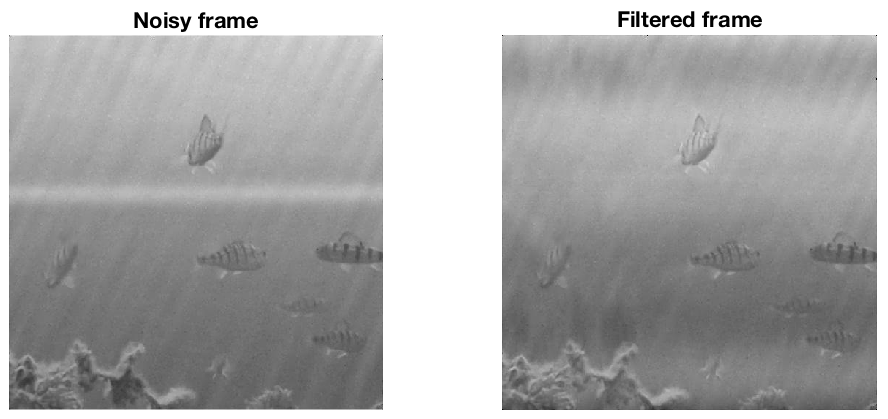
\includegraphics[width=0.5\textwidth]{3.png}
\end{figure}

\section{Conclusion}
After applying one spatial domain and two frequency domain filters along with the help of intensity transformations (thresholding) I have finally obtained the cleanest video which I will add to the directory. But if to look from the beginning right to the end which is the process that has taken a lot of time and energy you will observe such result:

\begin{figure}[h]
	\centering
	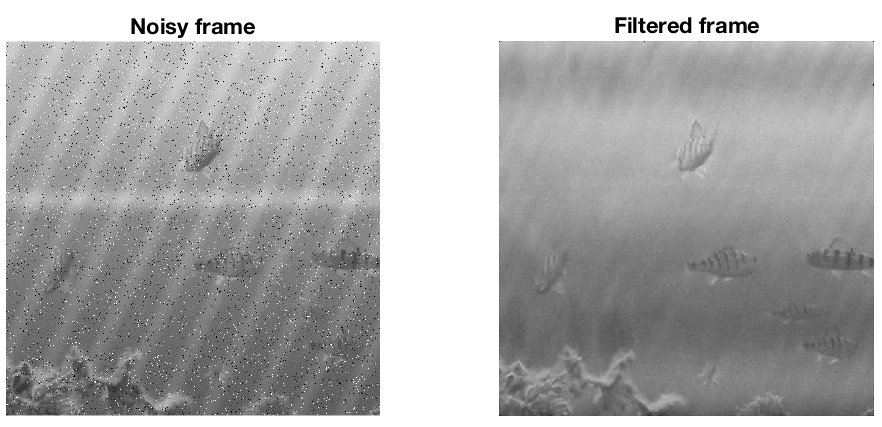
\includegraphics[width=0.5\textwidth]{final.png}
\end{figure}

\section{Acknowledgements}
By the end, I would like to thank teaching assistant Olzhas Adiyatov for his patience and great help in achieving the obtained result of the project. In addition, I would like to thank the authors of the book \textit{Signal Processing First} and professor Atakan Varol for suggesting this book. The book was used in understanding the nature of signals and frequency domain.

\end{document}